
\section*{Parte (d)}

\subsection*{(d)}
Corrija o problema identificado no item anterior e demonstre que a rede agora consegue aprender.

\vspace{0.5em}
\noindent De fato, adicionar um termo na inicialização dos parâmetros permitiu o aprendizado e subsequente redução da função perda. Isso ocorre pois o valor pelo qual multiplicamos os pesos iniciais é $(2/D)^{1/2}$, sendo $D$ o tamanho da camada. Isso reduz a variância dos parâmetros e evita que valores muito grandes sejam passados ao softmax e tenham seu gradiente próximo a zero.

\vspace{0.5em}
\noindent A correção implementada:

\begin{verbatim}
def init_scale(fan_in):
    return (2/fan_in)**0.5

# Inicialização com normalização adequada
A_K = torch.randn((D,D)).cuda() * init_scale(D)  # COM *init_scale(D)
A_Q = torch.randn((D,D)).cuda() * init_scale(D)  # COM *init_scale(D)
\end{verbatim}

\vspace{0.5em}
\noindent As evidências do aprendizado bem-sucedido incluem:

\begin{enumerate}
    \item \textbf{Redução da perda}: O gráfico da função perda agora mostra uma tendência decrescente clara ao longo das épocas.

    \item \textbf{Gradientes não-zero}: Os histogramas dos gradientes mostram distribuições mais amplas, indicando gradientes efetivos para o aprendizado.

    \item \textbf{Distribuição melhorada do softmax}: A saída do softmax apresenta uma distribuição mais balanceada, não saturada.
\end{enumerate}

\begin{figure}[h]
    \centering
    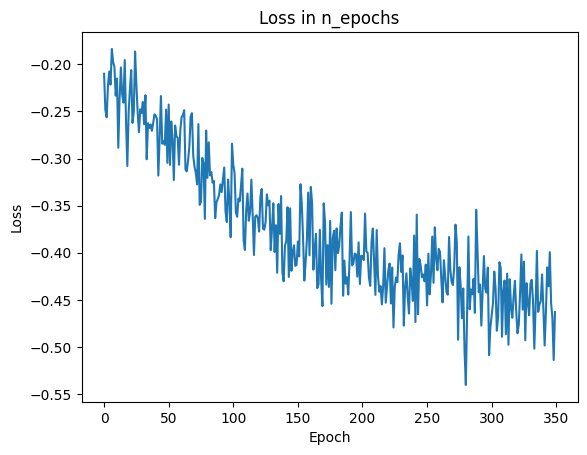
\includegraphics[width=0.7\textwidth]{../figures/4/loss_with_init_fix.png}
    \caption{Função perda com inicialização adequada - aprendizado bem-sucedido}
    \label{fig:loss_with_init}
\end{figure}

\begin{figure}[h]
    \centering
    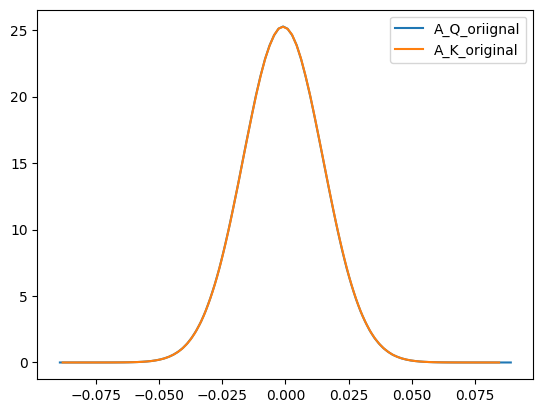
\includegraphics[width=0.7\textwidth]{../figures/4/weight_distributions_with_init_fix.png}
    \caption{Distribuições dos pesos iniciais A\_K e A\_Q com inicialização adequada}
    \label{fig:weights_with_init}
\end{figure}

\begin{figure}[h]
    \centering
    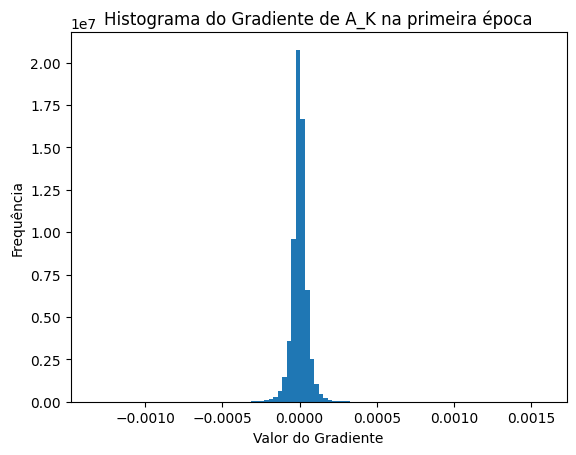
\includegraphics[width=0.45\textwidth]{../figures/4/gradient_histogram_A_K_with_init_fix.png}
    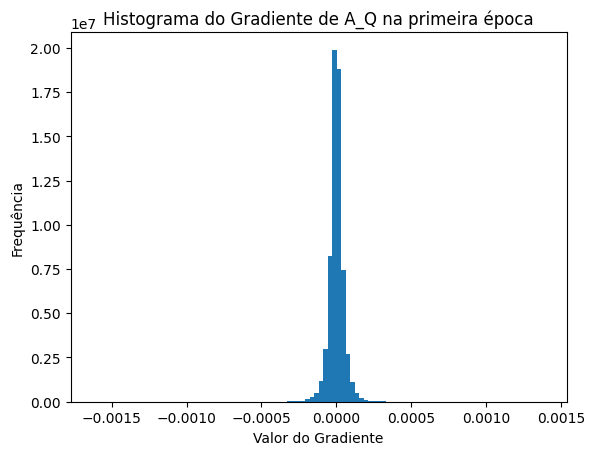
\includegraphics[width=0.45\textwidth]{../figures/4/gradient_histogram_A_Q_with_init_fix.png}
    \caption{Histogramas dos gradientes de A\_K e A\_Q na primeira época (com inicialização adequada)}
    \label{fig:gradients_with_init}
\end{figure}

\begin{figure}[h]
    \centering
    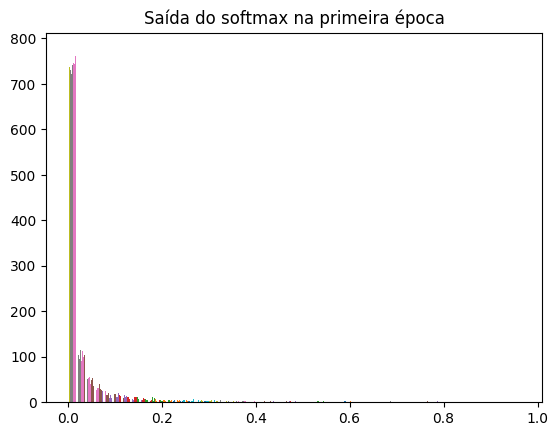
\includegraphics[width=0.7\textwidth]{../figures/4/softmax_output_with_init_fix.png}
    \caption{Saída do softmax na primeira época (com inicialização adequada)}
    \label{fig:softmax_with_init}
\end{figure}

